\documentclass[11pt]{article}

\usepackage{amsmath, amssymb, amsthm, amsfonts, mathtools}

\usepackage{graphicx}
\usepackage[hidelinks]{hyperref}
\usepackage{ifthen}
\usepackage{xcolor}
\usepackage{xspace}
\usepackage[skip=10pt]{caption}
\usepackage{geometry} % page layout
\usepackage{siunitx}
\geometry{a4paper, margin=1in}

\DeclareSIUnit\byte{B}
\DeclareSIUnit\bit{bit}
\DeclareSIUnit\petabyte{\peta\byte}
\DeclareSIUnit\gigabyte{\giga\byte}
\DeclareMathOperator{\round}{round}

% \usepackage{titlesec}
% \titlespacing*{\section}{0pt}{*2}{*1}

\theoremstyle{remark}
\newtheorem{remark}{Remark}

\title{Conjectures on the Period Lengths of One-Dimensional Cut-and-Project Sequences}
\author{Dirk Kunert \thanks{Independent Researcher, Email: dirk.kunert@gmail.com}}
\date{\today}

% TODO: See https://apps.hegl.mathi.uni-heidelberg.de/Proseminar-WS22-Quasicrystals/pages/cut-and-project1D.html


\begin{document}
%
% =================================================
\newcommand{\showfigures}{true}
\newcommand{\todo}[1]{\textcolor{red}{TODO: {#1}}}
\newcommand{\langc}[0]{\mbox{C}\xspace}
\newcommand{\langp}[0]{\mbox{Python}\xspace}
\newcommand{\chat}[0]{\mbox{\emph{ChatGPT o3-mini-high}}\xspace}
\newcommand{\function}[1]{\mbox{\texttt{#1}}\xspace}
% =================================================

\maketitle
%
\begin{abstract}
With $\alpha, \beta \in \mathbb{N}$, $\alpha \perp \beta$, $x, y \in \mathbb{R}$, $\omega \in \mathbb{R}_{\ge 0}$ and $i \in \mathbb{Z}$, we consider the points
%
\begin{equation}
\mathbf{P} 
= \left(
\begin{pmatrix} x \\ y \end{pmatrix}
\;\middle|\;
x \in \mathbb{Z},\,
y \in 
\left[\frac{\alpha}{\beta} (x - \omega),\; \frac{\alpha}{\beta} x + \omega\right] 
\cap \mathbb{Z}
\right)\label{eq:points}
\end{equation}
%
projected vertically onto $f(x) = \frac{\alpha}{\beta} x$ and measure their euclidian distances $\left( d^{(i)} \right)$.
%
With
\[
\Lambda_{\alpha, \beta} \;:=\; \alpha + \beta \;+\; 1,
\]
%
we propose the following conjectures concerning the period length $\lambda$ of $\left( d^{(i)} \right)$:
%
\begin{enumerate}
	\item \label{itm:conj1} There is always a finite $\lambda$.
 	\item \label{itm:conj2} If \(\omega \in (0,1)\), $\lambda_{\alpha, \beta} < \Lambda_{\alpha, \beta}$
 	\item \label{itm:conj3} If \(\omega = 1\), $\lambda_{\alpha, \beta} = \Lambda_{\alpha, \beta}$.
 	\item \label{itm:conj4} If \(\omega \in (1,2)\), $\lambda_{\alpha, \beta} \ge \Lambda_{\alpha, \beta}$
 	\item \label{itm:conj5} If \(\omega > 2\), $\lambda_{\alpha, \beta} > \Lambda_{\alpha, \beta}$
 	\item \label{itm:conj6} If \(\omega \ne 1\), $\lambda \approx \left\lfloor (\omega \; \Lambda_{\alpha, \beta} \right\rfloor$
\end{enumerate}
%
We use numerical methods to support these conjectures.
%
\begin{remark}
We will show, that $\lambda_{\omega = 0} = 1$.
\end{remark}
%
\begin{remark}
Conjecture~\ref{itm:conj6} is the result of a conversation with \chat.
\end{remark}
\end{abstract}

% ====================
\section{Introduction}
% ====================

In 2017, Yves Meyer (École Normale Supérieure Paris-Saclay, France) won the Abel Prize “for his pivotal role in the development of the mathematical theory of wavelets” (see \cite{AbelPriceYvesMeyer}).
%
Terence Tao (University of California, Los Angeles) held the announcement (see \cite{SpeechTao}) and presented Figure~\ref{fig:MeyerSets}.
%
\begin{figure}[htbp]
    \centering
    \ifthenelse{\equal{\showfigures}{true}}{
		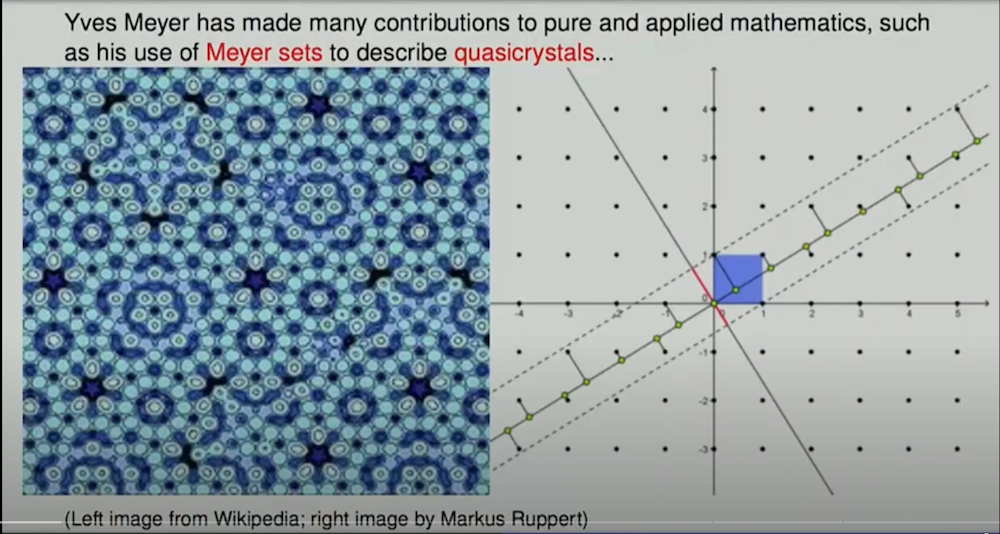
\includegraphics[width=0.8\textwidth]{cut_and_project_tao}
	}{
	}
    \caption{Screenshot from Terence Tao's presentation taken 60 seconds after the video's start}
    \label{fig:MeyerSets}
\end{figure}

Observing the distances of the points (see Figure~\ref{fig:MeyerSets}, right), he stated the following: "They repeat themselves, but not in a regular fashion."

These one-dimensional cut-and-project sequences are explored here. \langc and \langp software is used to support our conjectures (see \cite{Kunert2025}).

% ===============================
\section{Construction of the Set}
% ===============================

% =====================
\subsection{Projection}
% =====================

In Figure~\ref{fig:a2o1}, 
the function that is projected vertically onto is $f(x) = \frac{\alpha}{\beta} x$, 
the upper, passing through $(0, \omega)$, is given by $u(x) = \frac{\alpha}{\beta} x + \omega$, 
and the lower, passing through $(\omega, 0)$, by $l(x) = \frac{\alpha}{\beta} \, (x - \omega)$, 
with $x \in \mathbb{R}$, $\alpha, \beta \in \mathbb{N}$, and the offset $\omega \in \mathbb{R}_{\ge 0}$.

\begin{figure}[htbp]
    \centering
    \ifthenelse{\equal{\showfigures}{true}}{
		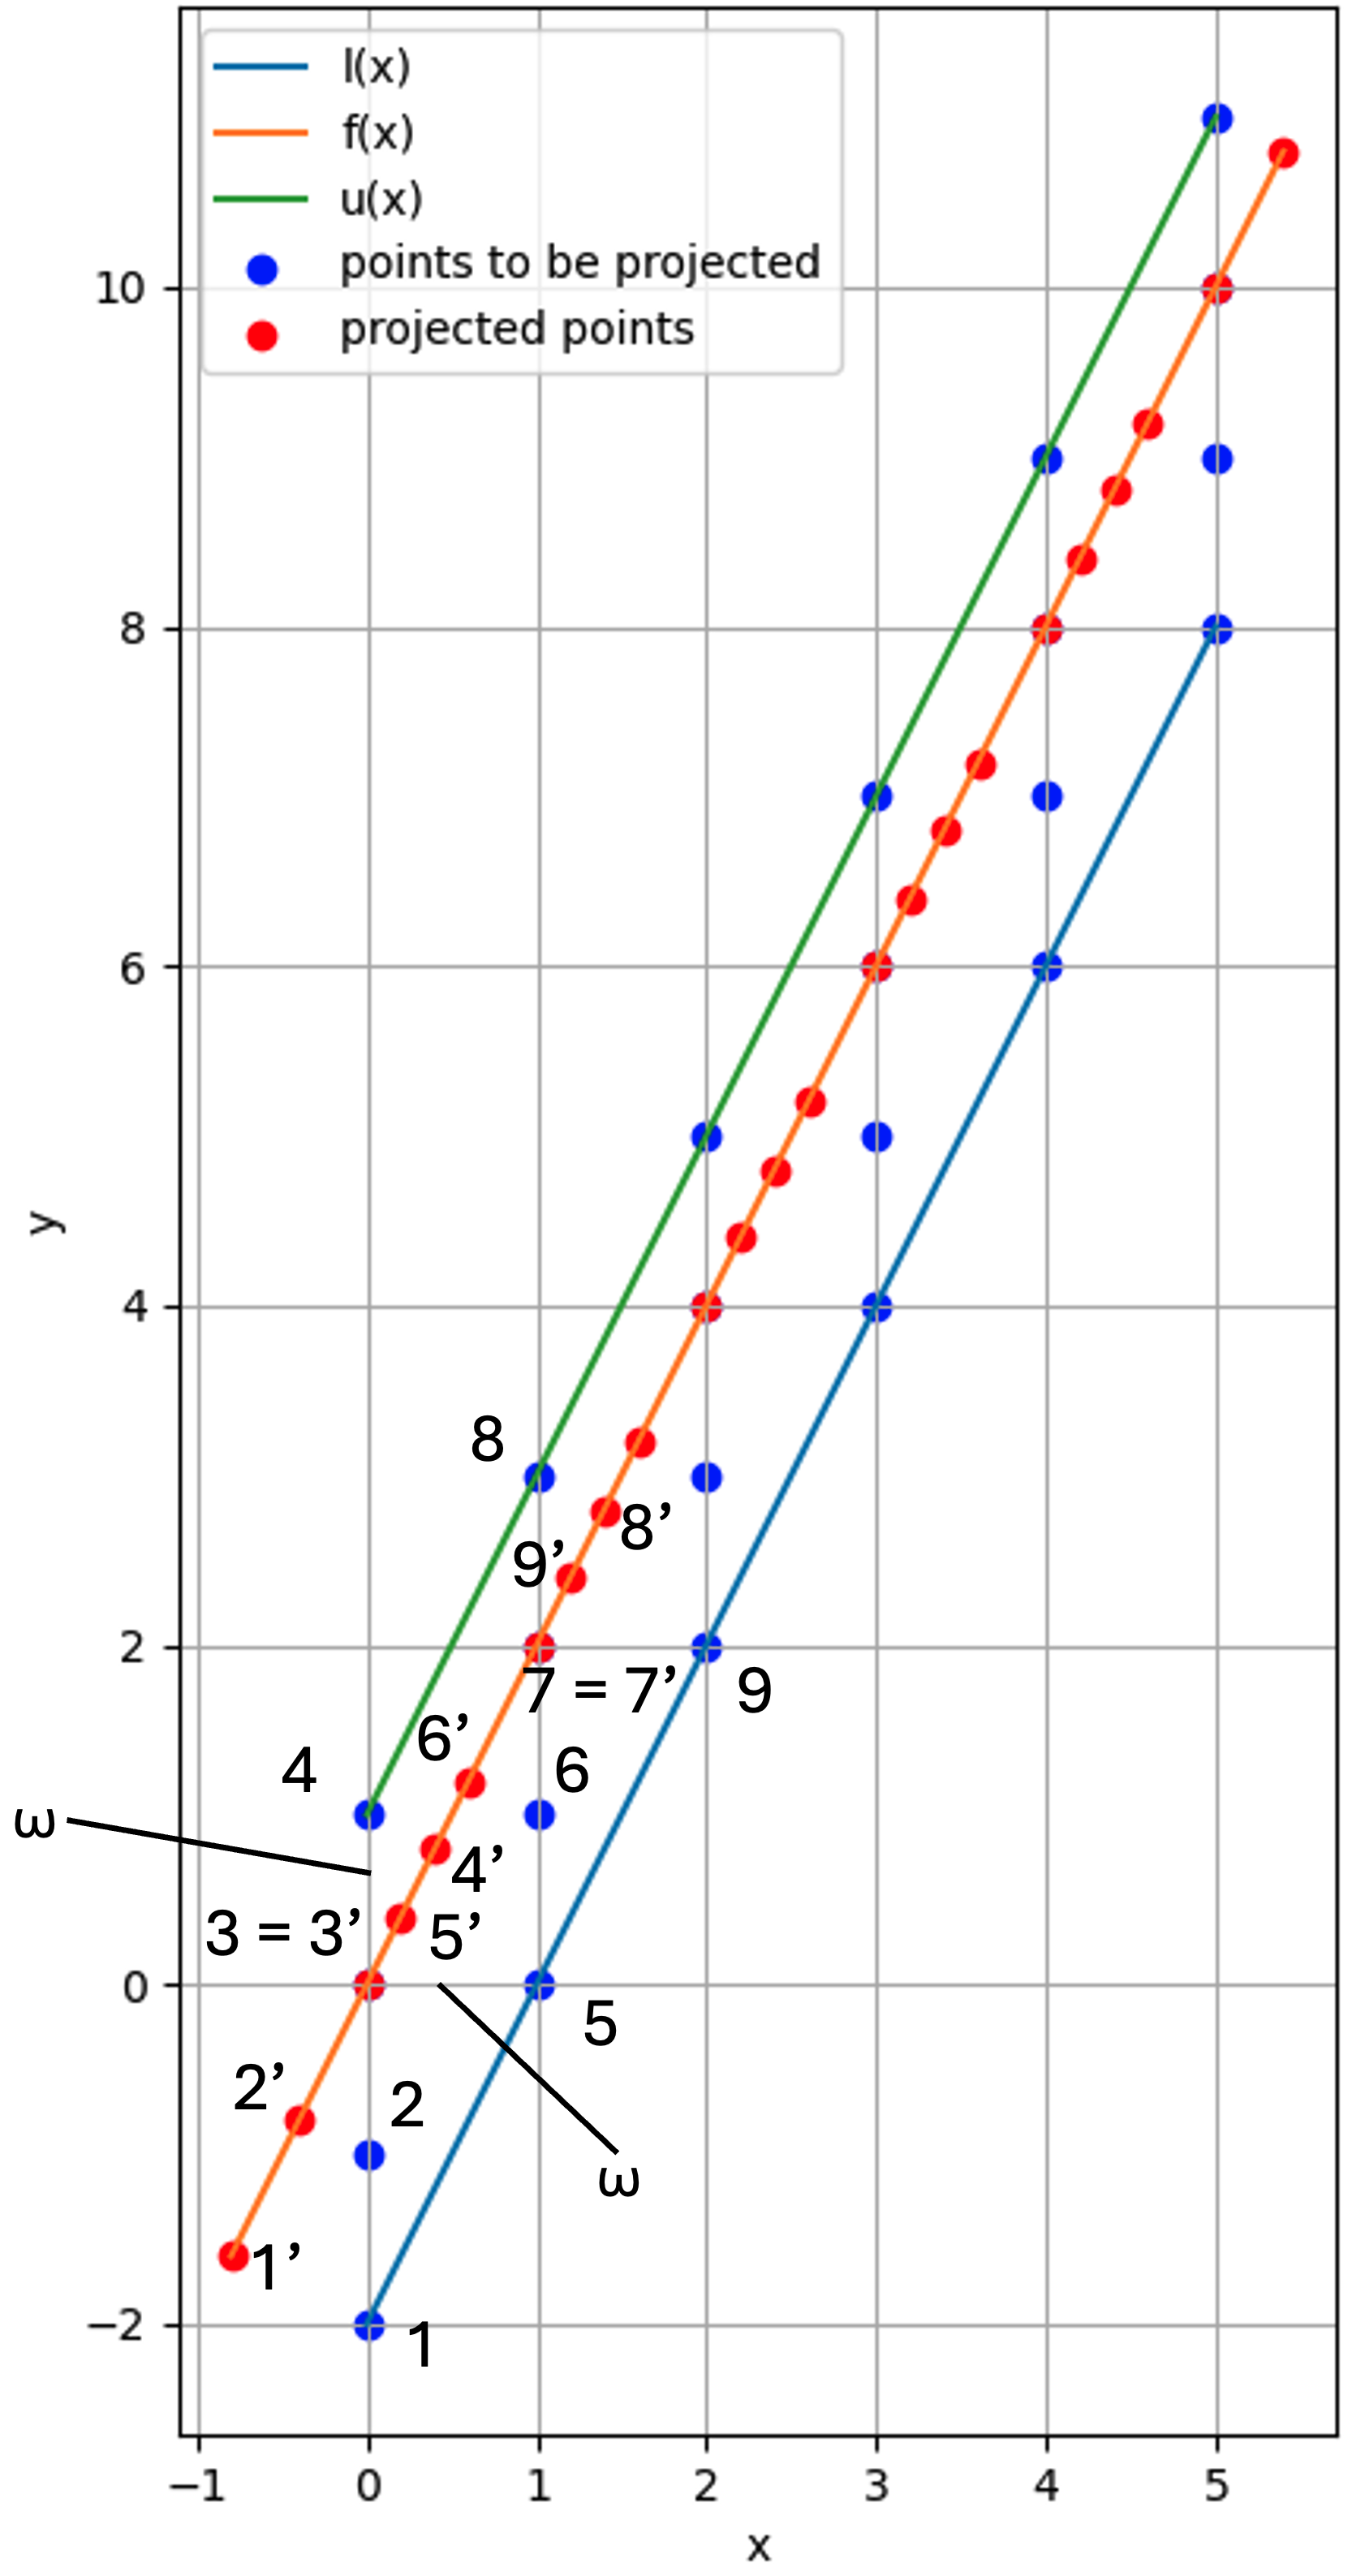
\includegraphics[width=0.4\textwidth]{a2o1}
	}{
	}
	\caption{Illustration of the projection of points for $\frac{\alpha}{\beta} = 2$ and $\omega = 1$ within the interval $[0, 5]$}
    \label{fig:a2o1}
\end{figure}
%
Projecting the points shown in equation \ref{eq:points} vertically on $f(x) = \frac{\alpha}{\beta} x$, we get
%
\begin{equation}
\mathbf{\tilde{P}}
= \frac{1}{\alpha^2 + \beta^2} \begin{pmatrix} \beta^2 & \alpha \beta \\ \alpha \beta & \alpha^2 \end{pmatrix} \mathbf{P}.\label{eq:c}
\end{equation}
%
Figure~\ref{fig:a2o1} shows that the first projected points are $1'$, $2'$, $3'$, $5'$, $4'$, $6'$, $7'$, $9'$, and $8'$. They are not in the correct order. So, $\mathbf{\tilde{P}}$ must be sorted by the x-coordinates of its points. We get
\begin{equation}
\mathbf{\tilde{P}}_s = \left(\mathbf{\tilde{p}}_s^{(i)} \right),\label{eq:sort}
\end{equation}
with $i \in \mathbb{Z}$.
%
\begin{remark}
We use $\mathbb{Z}$ instead of $\mathbb{N}$, because we have a "two-way infinite sequence" (see \cite{Senechal2009}, p.~106).
\end{remark}
%
\begin{remark}
Numerical experiments show, that sorting has no influence on $\lambda$.
\end{remark}
%
For the numerical analysis we limit $x$ to $[0, x_{max}]$, with $x_{max} \in \mathbb{N}$.
%
Examining Figure~\ref{fig:a2o1} again, we observe the following squared distances:
%
\begin{table}[htbp]
\centering
\begin{tabular}{| c | c || c | c | c | c | c | c | c | c | c | c || c |}
    \hline
    \textbf{Index} &   1 &   2 &   3 &    4 &   5 & \dots &  18 &  19 &   20 &  21 &  22 &  23 \\ \hline
    \textbf{Value} & 0.8 & 0.8 & 0.2 & 1.48 & 0.2 & \dots & 0.8 & 0.2 & 1.48 & 0.2 & 0.8 & 0.8 \\ \hline
\end{tabular}
\caption{Squared distances in Figure~\ref{fig:a2o1} for $x_{max} = 5$}
\label{tab:distances1}
\end{table}

By choosing the interval $[0, 5]$, $0.8$ is added at the beginning and at the end, making the sequence appear non-periodic despite the repetition of $(0.8, 0.2, 1.48, 0.2)$. Indeed, if we choose the interval $[0, 10]$, the series continues as expected:
%
\begin{table}[htbp]
\centering
  \begin{tabular}{| c | c | c | c | c | c | c |}
    \hline
    \textbf{Index} & \dots &  22 &  23 &   24 &  25 & \dots \\ \hline
    \textbf{Value} & \dots & 0.8 & 0.2 & 1.48 & 0.2 & \dots \\ \hline
  \end{tabular}
\caption{Squared distances in Figure~\ref{fig:a2o1} for $x_{max} = 10$}
\label{tab:distances2}
\end{table}

To solve this problem in the numerical experiments, we delete elements from the beginning and the end of $P_s$, while no finite $\lambda$ is found. We limit the number of removed elements to 10\% of the sequence length.
%
This way we get $K$ projected points.

% ===============================
\subsection{Distance Calculation}
% ===============================

The following applies to the euclidian distances of the ordered projected points with $\tilde{p}_{x s}^{(i)} \in [0, x_{max}]$:
%
\begin{equation}
\left( d^{(i)} \right)_{i=1}^{K-1} = \left\lVert \mathbf{\tilde{p}}^{(i+1)}_s - \mathbf{\tilde{p}}^{(i)}_s \right\rVert
\end{equation}
%
Every injective function applied to the elements of $\left(d^{(i)}\right)_{i=1}^{K-1}$ does not change $\lambda$.
%
$f(x) = x^2$ is injective for $x \in \mathbb{R}_{\geq 0}$. Thus, we can use the squared distances $\left(s^{(i)}\right)_{i=1}^{K-1}$ instead of the euclidian ones:
%
\begin{align}
s^{(i)} &= \left(\tilde{p}_{x s}^{(i+1)} - \tilde{p}_{x s}^{(i)}\right)^2 + \left(\tilde{p}_{y s}^{(i+1)} - \tilde{p}_{y s}^{(i)}\right)^2 \\
                                 &= \left(1 + \frac{\alpha^2}{\beta^2} \right) \left(\tilde{p}_{x s}^{(i+1)} - \tilde{p}_{x s}^{(i)}\right)^2,
\end{align}
%
because
%
\begin{equation}
\tilde{p}_{y s}^{(i)} = \frac{\alpha}{\beta} \tilde{p}_{x s}^{(i)}.
\end{equation}
%
$f(x) = \gamma x$ and $f(x) = \sqrt{x}$ are injective for $\gamma \in \mathbb{R}_{\ne 0}$ and $x \in \mathbb{R}_{\geq 0}$ as well. We get
%
\begin{equation}
\tilde{s}^{(i)} = \left(\tilde{p}_{x s}^{(i+1)} - \tilde{p}_{x s}^{(i)}\right).
\end{equation}
%
From equation~\eqref{eq:c} it follows that
%
\begin{equation}
\tilde{p}_{x s}^{(i)} = \frac{\beta}{\alpha^2 + \beta^2} \left( \beta p_{x s}^{(i)} + \alpha p_{y s}^{(i)} \right).
\end{equation}
%
Here we also can omit the constant $\frac{\beta}{\alpha^2 + \beta^2}$. Finally, we obtain
%
\begin{equation}
\left(\delta^{(i)}\right)_{i=1}^{K-1} =
\left( 
	\beta \left( p_{x s}^{(i+1)} - p_{x s}^{(i+1)} \right)
	+ \alpha \left( p_{y s}^{(i+1)} - p_{y s}^{(i+1)} \right) 
\right)_{i=1}^{K-1}.
\label{delta}
\end{equation}
%
This sequence is now examined for periodicity.

\begin{remark}
$\tilde{p}_{x s}^{(i)} = \tilde{p}_{x s}^{(j)}$ for $i, j \in \mathbb{Z}$ and $i \ne j$ may occur under specific conditions: For $\frac{\alpha}{\beta} = 1$ and $\omega = 1$ both points, $(0, 1)$ and $(1, 0)$, are projected to $(0.5, 0.5)$. Therefore $\left(\delta^{(i)}\right)_{i=1}^{K-1}$ is not discrete.
\end{remark}

% ===================
\section{Periodicity}
% ===================

We consider the finite sequence $\left(e^{(i)}\right)_{i=1}^{L}$ with $L \in \mathbb{N}_{>1}$ to be periodic, if there exists a $\tilde{\lambda} \in [1, L//2]$ with 
%
\begin{equation}
e^{(i+\tilde{\lambda})} = e^{(i)} \; \forall i \in [1, L-\tilde{\lambda}].
\end{equation}
%
The period length $\lambda$ is defined as
%
\begin{equation}
\lambda := \min\left(\tilde{\lambda}^{(i)} \right).
\end{equation}
%
\begin{proof}
$\lambda_{\omega = 0} = 1$: As sorting is not necessary, $\mathbf{P}_s = \mathbf{P}$. Thus,
%
\begin{equation}
\left(\delta^{(i)}\right)_{i=1}^{K-1} = \left(\beta \left(p_x^{(i+1)} - p_x^{(i)}\right) + \alpha \left(p_y^{(i+1)} - p_y^{(i)}\right)\right)_{i=1}^{K-1}
\end{equation}
%
according to \ref{delta}. As $p_x^{(i+1)} - p_x^{(i)} = 1$ and $p_y^{(i+1)} - p_y^{(i)} = \frac{\alpha}{\beta}$, we get
\begin{equation}
\left(\delta^{(i)}\right)_{i=1}^{K-1} = \left(\beta + \frac{\alpha^2}{\beta}\right)_{i=1}^{K-1},
\end{equation}
%
which consists of constant elements. As $e^{(i+1)} = e^{(i)} \; \forall i \in [1, K-2]$, $\lambda_{\omega = 0} = 1$.
\end{proof}

% ===================
\section{Conjectures}
% ===================

In very rare cases, we see that our \langc software is not able to calculate a finite period length because the size of the array containing the differences is not sufficient. This array consists of 8,000,000,000 elements with \SI{64}{\bit} and has a size of more than \SI{60}{\gigabyte}.

\subsection{Conjectures 1 to 5}

Using the \langc software, we were able to support all conjectures listed in the abstract.

\begin{remark}
The fraction for $a = \sqrt{2}$, represented with \SI{64}{\bit} floating-point arithmetic, is
%
\begin{equation}
\tilde{a} = \frac{6{,}369{,}051{,}672{,}525{,}773}{4{,}503{,}599{,}627{,}370{,}496}.
\end{equation}
%
If conjecture~\ref{itm:conj3} is correct, we would obtain
%
\begin{equation}
\lambda_{a = \tilde{a}, \; \omega = 1} = 10{,}872{,}651{,}299{,}896{,}270.
\end{equation}
%
Such a sequence with \SI{8}{\bit} per element would take up around \SI{11}{\petabyte} of memory.
Provided conjecture~\ref{itm:conj3} was correct, there is no finite $\lambda$, because $\sqrt{2}$ can only be represented by infinitely large numerators and denominators.
\end{remark}

\subsection{Conjecture \ref{itm:conj6}}

We found conjecture~\ref{itm:conj6} by providing \emph{ChatGPT o3-mini-high} data created by the \langc function \function{create\_test\_data} and telling it, it should use \emph{XGBoost} to predict $\lambda$. It created the \langp function \function{xgboost} (see \cite{Kunert2025}). 

When we sent ChatGPT the result of this computation, it wrote of an ”indication that the four predictors \(o_n, o_d, a_n, a_d\) [$\omega = \frac{o_n}{o_d}$, $\alpha = a_n$ and $\beta = a_d$] are in a highly complex, non-linear relationship, which XGBoost captures excellently". Then we reported on conjecture~\ref{itm:conj3} and told \chat, that we want to find a formula for $\lambda$.

Among other suggestions, it proposed the following:
%
\begin{equation}
\lambda = \omega \; \Lambda_{\alpha, \beta}
\end{equation}

By experimenting with the \langc software we found that
%
\begin{equation}
\lambda = \left\lfloor \omega \; \Lambda_{\alpha, \beta} \right\rfloor
\end{equation}
%
gives even better results. The lowest value we found for $R^2$ with the \langc function \function{test\_conjectures} was $0.987994$.

% =========================
\begin{thebibliography}{99}
% =========================

\bibitem{AbelPriceYvesMeyer}
\emph{Page for Yves Meyer at the Abel Prize Homepage}, available at: 
\url{https://abelprize.no/abel-prize-laureates/2017}, accessed on December 15, 2024.

\bibitem{SpeechTao}
\emph{Terence Tao on Yves Meyer's work on Wavelets}, available at: 
\url{https://youtu.be/AnkinNVPjyw}, accessed on December 15, 2024.

%\bibitem{BaakeGrimm2013}
%Michael Baake and Uwe Grimm
%\textit{Aperiodic Order: Volume 1, A Mathematical Invitation},
%2013.
%ISBN: 978-0521869911.

\bibitem{Senechal2009}
Marjorie Senechal,
\emph{Quasicrystals and geometry},
2009.
ISBN: 978-0-521-57541-6.

\bibitem{Kunert2025}%
D.\,Kunert, 2025,
\emph{Code for this article},
Available at \url{https://github.com/dkunert/cut-and-project/tree/main/src}.\\
\todo{Upload the code and this file!}

\end{thebibliography}

\section{Conclusion}
\todo{Missing!}

\end{document}